\documentclass{article}
\usepackage[utf8]{inputenc}
\usepackage{amsmath}
\usepackage{amsfonts}
\usepackage{amssymb}
\usepackage{polski}
\usepackage{indentfirst}
\usepackage{graphicx}
\usepackage{pdfpages}
\usepackage{gauss}
%script adding bars in matrix
\usepackage{etoolbox}
\makeatletter
\patchcmd\g@matrix
 {\vbox\bgroup}
 {\vbox\bgroup\normalbaselines}% restore the standard baselineskip
 {}{}
\makeatother

\newcommand{\BAR}{%
  \hspace{-\arraycolsep}%
  \strut\vrule % the `\vrule` is as high and deep as a strut
  \hspace{-\arraycolsep}%
}


\begin{document}
\title{Sprawozdanie-Metody numeryczne i optymailzacja}
\author{Jakub Andryszczak 259519,\\ Jakub Żak 244255,\\ Maciej Cierpisz 249163}
\date{}
\maketitle
\tableofcontents
\newpage
%Tutaj zaczyna się wstęp
\section{Wstęp}
Mieliśmy do rozwiązania problem, który polegał na tym, że po otrzymaniu sygnału z anten sieci komórkowej musieliśmy zlokalizować dany telefon w budynku wydziału MiNI. Do określenia były współrzędne x, y oraz piętro w budynku.\\

Projekt ten wykonywaliśmy w ośmioosobowej grupie. Co tydzień spotykaliśmy się na zajęciach, gdzie omawialiśmy postępy w zadaniu i stawialiśmy sobie nowe cele, zadania, a także rozpatrywaliśmy potencjalne problemy. Stworzyliśmy także grupę dyskusyjną, gdzie omawialiśmy rezultaty działań i zawieraliśmy istotne spostrzeżenia nt. projektu. Powstała również wspólna przestrzeń dyskowa, gdzie udostępnialiśmy sobie nawzajem różne dane, skrypty, wyniki, informacje, dokumenty, poradniki, wykresy i statystyki.\\

Do próby rozwiązania problemu wykorzystaliśmy uczenie maszynowe. Używaliśmy oprogramowania RapidMiner.

%Tu chce mieć obrazek
\begin{figure}[h!]
\centering

\end{figure}
Pomocny również okazał się program MATLAB, w którym pisaliśmy pomocne skrypty takie jak:\\%DOKOŃCZYC
\begin{itemize}
\item Generator trójwymiarowych map, które pokazywały rozkładanie się błędu na współrzędnych x i y
\item Generator twójwymiarowych map siły sygnału z anteny
\item `Wycięcie' prostopadłościanu danych
\item Wartościowanie anten
\end{itemize}
Dokładniejszy opis powyższych skryptów został zamieszczony w rozdziale trzecim. 

%Koniec wstępu
\section{Pierwsze próby}
Za cel postawiliśmy sobie uzyskanie klasyfikatora, który dla wektora pomiarów ustala piętro, na którym mogły zostać wykonane.

Wykonaliśmy wstępną analizę danych, zbadaliśmy osiągi różnych klasyfikatorów dla pierwotnej postaci danych. Nastęnie okazało się, że należy na nie nanieść różne poprawki, niezbędne do dalszych badań. Szczególny problem okazał się z niefortunnie dobraną wartością $-1$ jako oznaczeniem braku sygnału z danej anteny. Wartość tą zmienialiśmy na $-200$ (próby użycia innych wartosci dawały nielepsze rezultaty), ponieważ siła sygnału słabła wraz ze spadkiem tej wartości.

Następnie została wybrana maszyna wektorów nośnych (SVM) z funkcją Gaussa jako funkcją jądrową, ponieważ dawała nam ona najbardziej obiecujące wyniki przy klasyfikacji piętra.

Michał Kowalkowski zajmował się próbą aproksymacji położenia z użyciem SVM, kNN, sieci neuronowych. Jednak i najlepsze wyniki uzyskał podczas pracy z SVMem z jądrem anova.

Wykonano optymalizację parametrów uczenia (w oparciu o wyniki uzyskane w walidacji krzyżowej). Później testowano także różne strategie transformacji danych (przeskalowania pomiarów, poprawki związane z logarytmiczną naturą głośności sygnału, odrzucania pomiarów nieprzekraczających pewnych progów, etc.)  Niestety nie miało to istotnego wpływu na wyniki.

\section{Praca na danych z MATLABem}

Na samym początku zespół Kuby i Dawida zrobił trójwymiarowe mapy w programie MATLAB pokazujące, jak rozkłada się błąd względny na współrzędnych x i y (oddzielnie) dla wszystkich punktów na wydziale dla każdej anteny. Dopasowano kolory (zielony, żółty, czerwony i czarny dla braku sygnału) punktów pomiarów tak, aby było to czytelne i można było dokonać stosownej analizy.
Dodatkowo stworzono także mapy błędów w zależności od piętra (oznaczenia podobne jak wcześniej - zielony kolor punktu oznaczał wyznaczenie dobrego piętra, żółty -jedno piętro różnicy, czerwony - różnia większa).\\

Oprócz błędów, wykonali także trójwymiarowe mapki siły sygnału z anteny.
Badanie map błędów i map sił sygnałów pozwoliło jedynie stwierdzić, że błąd w lokalizacji był największy na tych obszarach, gdzie dominuje słaby sygnał.\\

Warto też wspomnieć o tym, że stworzyli dodatkowo wykres słupkowy, w którym do każdej z anten przyporządkowano sumę sił wszystkich sygnałów odbieranych z tej anteny - to służyło do zorientowania się, czy z danej anteny uzyskano w ogóle jakiś sygnał i jakiej mógł on być jakości. Grupa od uczenia maszynowego początkowo przy klasyfikacji bazowała właśnie na tym, tj. wybierali te anteny, z których był stosunkowo silny sygnał.\\

\subsection{Wycięcie prostopadłościanu z danych}

Dawid wyciął z danych prostopadłościan (głównie punkty w okolicy klatki schodowej, usunięte sale z 2. piętra) i stworzył z tego nowy plik z danymi. Miało to służyć sprawdzeniu czy upodobnienie kształtu otoczki punktów, gdzie wykonywano pomiary, do prostopadłościanu, może poprawić osiagane wyniki.\\

\subsection{Wartościowanie anten}

Innym zadaniem zespołu była analiza danych celem wyboru anten, których odbierany sygnał rozchodził się monotonicznie w ramach jednej osi. To zdecydowanie ułatwiłoby poprawną lokalizację. Wobec tego należało wprowadzić pewną funkcję wartościującą dla każdej z anteny, aby móc wybrać te, dla których można by z klasyfikacji uzyskać znacznie lepsze wyniki.\\

W MATLABie wyznaczenie wartości rankingowej polegało na:\\
\begin{enumerate}
\item
wybraniu wszystkich pomiarów w danym punkcie i stworzeniu unikalnego rekordu (te same współrzędne), gdzie mocą anten w tym przypadku była mediana wszystkich mocy sygnałów z każdego punktu - uznaliśmy, że taki model pozwoli na złagodzenie ewentualnych różnic w przypadku wielokrotnych pomiarów
\item
następnie należało sprawdzić, jak sygnał zachowuje się w swoistych “tunelach”, czyli jak zachowuje się on wzdłuż którejś z osi (\textit{OX,OY,OZ}) dla ustalonych dwóch współrzędnych niezależnych od przyjętej osi.\\
\end{enumerate}
Chcieliśmy, by sygnał (w miarę) równomiernie malał albo rósł. Kornel wymyślił sposób, który następnie został zaimplementowany, by liczyć wartość spadków sygnału pomiędzy punktami w sekwencji (na przykład w przypadku pionu spadek sygnału pomiędzy kolejnymi dwoma piętrami) i ilość wzrostów, a następnie bezwzględną różnicę tych wartości. To powodowało, że dla sygnału mniej więcej monotonicznego (czyli dobrego w naszym przypadku) wartość ta była duża, bo był spory wzrost/spadek i bardzo mały spadek/wzrost. Dla sygnału w kształcie "piły zębatej" czy też stałej wartości - w tym przypadku spadki i wzrosty były podobne, dlatego różnica bezwzględna niwelowała to do niemalże zera. Wartością rankingową anten była suma tych różnic po wszystkich punktach (dla pionu po wszystkich x,y).\\
Co więcej, można zauważyć, że w przypadku braku odbioru sygnału dla dużej ilości punktów wartościowanie będzie niewielkie.
Oczywiście zdawaliśmy sobie sprawę, że takie podejście może nie uwzględnić niektórych szczególnych anten, dla których niskie wartościowanie wynika nie ze źle rozchodzącego się sygnału, ale z małej ilości punktów, dla których odebrano sygnał.
Wobec tego zastosowaliśmy pomocniczą wartość - maksymalną różnicę w ramach jednego "tunelu", która mogła pomóc w znalezieniu właśnie takich anten i ewentualnym uwzględnieniu ich w procesie uczenia maszynowego.
\\

Mimo wykorzystania tak wyznaczonych rankingów anten do selekcji cech, udało się tylko w niewielkim stopniu polepszyć uzyskiwane wyniki.

%Tutaj obrazek Kuby (wykres który jest w pliku drive


\section{Szukanie klasyfikatora piętra}
Po uzyskaniu początkowo nieobiecujących wyników, zajęliśmy się problemem kategoryzacji anten pod względem różnicy sił sygnałów (zwłaszcza na poszczególnych piętrach). Korzystaliśmy w tym celu z MATLABa generując mapy, które dały nam obraz tego, że w większości wypadków sygnał rozchodzi się na tyle "kuliście" na przestrzeni pięter, że podobne odczyty daje na skrajnych poziomach. To potwierdziły testy na maszynach w Rapidminerze, bo klasyfikator pietra bardzo często mylił własnie poziomy, które nie sąsiadowały ze sobą, a były równo oddalone od pewnego punktu (np. piętro pierwsze mylone było z piątym).

Później podejmowaliśmy eksperymenty w Rapidminerze na różnych maszynach pod kątem właśnie klasyfikacji piętra i sprawdzaliśmy jak zachowywały się wyniki przy różnych algorytmach wybierania anten (wyrzucania szumiących i zostawiania tych z dużymi róznicami pomiędzy poziomami), ale niestety nie miało to praktycznie żadnego wpływu na wynik. Próbowaliśmy też wykonać ręczną selekcję cech na podstawie przeciętnej jakości sygnału z danej anteny (nie udało się, wyniki były nielepsze niż uzyskane wcześniej).

Jednocześnie próbowaliśmy zmiany podejścia i wytrenowania klasyfikatora nie piętra, a pomieszczenia. To nie dało żadnych praktycznie użytecznych wyników. Warto jednak zwrócić uwagę na fakt, że im bardzo kształt pomieszczenia jest zbliżony do kwadratu (pod warunkiem, że jest tam wystarczająco wiele punktów pomiarowych) tym skuteczniej klasyfikator ,,przypomina sobie'' dane pomieszczenie. Do rozważenia jest opcja sztucznego podziału budynku na kwadraty i klasyfikowanie kwadratów, żeby wewnątrz nich uszczegółowić wynik.

Należy też zwrócić uwagę na fakt, że dla takiej charakterystyki danych korzystanie z metody kNN prawie automatycznie powoduje "przeuczenie" na zbiór uczący, z uwagi na bardzo dużą liczbę pomiarów w każdym z punktów.
\\
\\
\section{Zadanie nr. 1}
Rozwiązać ręcznie i komputerowo metodą eliminacji Gaussa poniższy układ równań
liniowych. Znaleźć elementy podstawowe (pivots).

\begin{equation}
    \begin{cases}
      2u-v=0 \\
     -u+2v-w=0 \\
     -v+2w-z = 0 \\
     -w+2z=5
    \end{cases}\,.
\end{equation}
\pagebreak

Do wykonania tego zadania rozpisano lewą stronę jako macierz 4x4 oraz wektor wynikowy 1x4

\[
  \linespread{2}\selectfont
  \addtolength{\arraycolsep}{10pt}
 \begin{gmatrix}[b]
2 & -1 & 0 & 0 & \BAR & 0\\
-1 & 2 & -1 & 0 & \BAR & 0\\
0 & -1 & 2 &-1 & \BAR & 0\\
0 & 0 & -1 & 2 & \BAR & 5
 \rowops
 \add[\cdot \frac1{2}]01
 %\mult{3}{\cdot \left(-\frac2{29}\right)}

 \end{gmatrix}
\]

\[
  \linespread{2}\selectfont
  \addtolength{\arraycolsep}{10pt}
 \begin{gmatrix}[b]
2 & -1 & 0 & 0 & \BAR & 0\\
0 & \frac3{2} & -1 & 0 & \BAR & 0\\
0 & -1 & 2 &-1 & \BAR & 0\\
0 & 0 & -1 & 2 & \BAR & 5
 \rowops
 \add[\cdot \frac2{3}]12
 %\mult{3}{\cdot \left(-\frac2{29}\right)}

 \end{gmatrix}
\]

\[
  \centering
  \linespread{2}\selectfont
  \addtolength{\arraycolsep}{10pt}
 \begin{gmatrix}[b]
2 & -1 & 0 & 0 & \BAR & 0\\
0 & \frac3{2} & -1 & 0 & \BAR & 0\\
0 & 0 & \frac4{3} &-1 & \BAR & 0\\
0 & 0 & -1 & 2 & \BAR & 5
 \rowops
 \add[\cdot \frac3{4}]23
 %\mult{3}{\cdot \left(-\frac2{29}\right)}

 \end{gmatrix}
\]

\[
  \centering
  \linespread{2}\selectfont
  \addtolength{\arraycolsep}{10pt}
 \begin{gmatrix}[b]
2 & -1 & 0 & 0 & \BAR & 0\\
0 & \frac3{2} & -1 & 0 & \BAR & 0\\
0 & 0 & \frac4{3} &-1 & \BAR & 0\\
0 & 0 & 0 & \frac5{4} & \BAR & 5
 \rowops
 \mult{3}{\cdot \left(-\frac4{5}\right)}
 \add[]23
 \end{gmatrix}
\]

\[
  \centering
  \linespread{2}\selectfont
  \addtolength{\arraycolsep}{10pt}
 \begin{gmatrix}[b]
2 & -1 & 0 & 0 & \BAR & 0\\
0 & \frac3{2} & -1 & 0 & \BAR & 0\\
0 & 0 & \frac4{3} & 0 & \BAR & 4\\
0 & 0 & 0 & 1 & \BAR & 4
 \end{gmatrix}
\]

\[
  \centering
  \linespread{2}\selectfont
  \addtolength{\arraycolsep}{10pt}
 \begin{gmatrix}[b]
2 & -1 & 0 & 0 & \BAR & 0\\
0 & \frac3{2} & 0 & 0 & \BAR & 3\\
0 & 0 & 1 & 0 & \BAR & 3\\
0 & 0 & 0 & 1 & \BAR & 4
 \end{gmatrix}
\]

\[
  \centering
  \linespread{2}\selectfont
  \addtolength{\arraycolsep}{10pt}
 \begin{gmatrix}[b]
2 & 0 & 0 & 0 & \BAR & 2\\
0 & 1 & 0 & 0 & \BAR & 2\\
0 & 0 & 1 & 0 & \BAR & 3\\
0 & 0 & 0 & 1 & \BAR & 4
 \end{gmatrix}
\]

\[
  \centering
  \linespread{2}\selectfont
  \addtolength{\arraycolsep}{10pt}
 \begin{gmatrix}[b]
1 & 0 & 0 & 0 & \BAR & 1\\
0 & 1 & 0 & 0 & \BAR & 2\\
0 & 0 & 1 & 0 & \BAR & 3\\
0 & 0 & 0 & 1 & \BAR & 4
 \end{gmatrix}
\]

\section{Zadanie nr. 5}
Zadanie nr. 5 polegało na zaimplementowaniu dowolnego algorytmu do faktoryzacji LU i zastosowaniu do zadanej macierzy. Zdecydowano się na algorytm Crout. Poniżej implementacja algorytmu na zadanej macierzy.\\
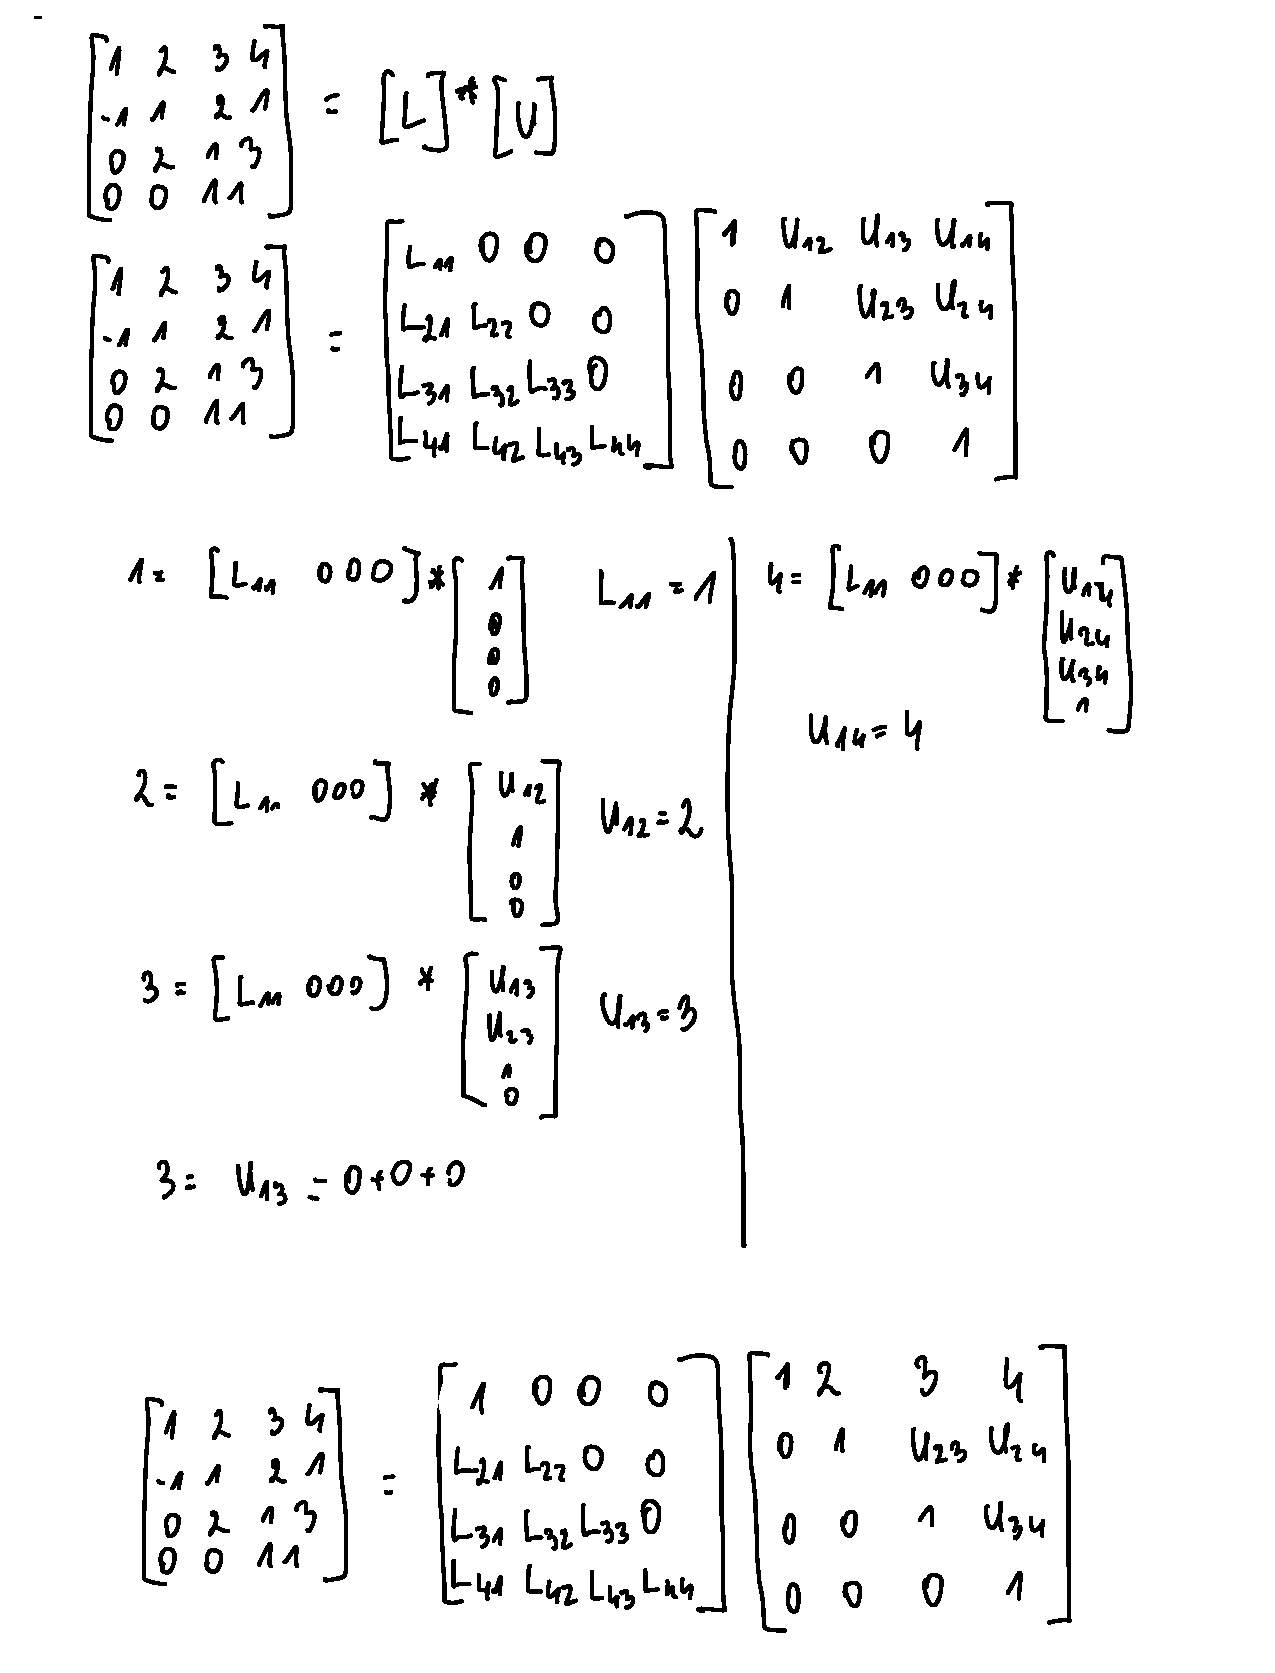
\includepdf[pages=-]{zad5.pdf}
\section{Selekcja cech}

Opracowana metody rankingowania anten oddzielnie dla każdej osi budynku, z uwzględnieniem monotoniczności jego rozchodzenia się w tej osi, wykorzystana do selekcji cech dla SVM, ostatecznie pozwoliła na uzyskanie najwyższej dotąd skuteczności klasyfikacji piętra na poziomie niecałych 54\%.
Rozważono dodatkową hipotezę - scenariusz gdzie w “rogach” budynku (wierzchołkach prostopadłościanu) umieszcza się AP WiFi i wykorzystuje sygnał z nich jako dodatkową cechę. Co zaskakujące, nie zaowocowało to istotnie lepszym wynikiem (choć może przy dodatkowym nakłądzie pracy można by liczyć na więcej).


\section{Zakończenie}
Realizacja tego projektu była bardzo pouczająca. Dała nam ona podstawowy przegląd technik uczenia maszynowego (pojęcia takie jak SVM, kroswalidacja itp.), pokazała nam potęgę programu RapidMiner i nauczyliśmy się korzystać z jego podstawowych funkcji. Podczas jednych ćwiczeń przeprowadziliśmy eksperyment wspólnego rozpatrywania problemu (nie związanego z naszym projektem) - rozbitków na oceanie. Dzięki tym ćwiczeniom doszliśmy do wniosku, że wspólna analiza wszystkich pomysłów może być bardzo efektywna i przynieść znaczący postęp. Podsumowując, wykonanie projektu było ciekawym doświadczeniem, jednak niestety nie udało nam się go rozwinąć tak, aby nasze rozwiązanie mogło być wykorzystane w praktyce. Być może inne metody (takie jak wykorzystanie więcej niż jednego pomiaru do lokalizacji użytkownika) mogą dać lepsze wyniki, uważamy jednak, że dotarliśmy do granic możliwości zadanego podejścia. 
\end{document} 